\begin{center}
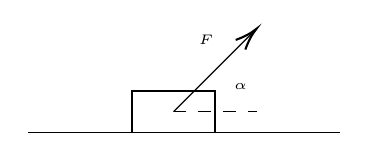
\begin{tikzpicture}[x=0.75pt,y=0.75pt,yscale=-1,xscale=1]
%uncomment if require: \path (0,300); %set diagram left start at 0, and has height of 300

%Straight Lines [id:da945561223656612] 
\draw    (160,150) -- (310,150) ;
%Shape: Rectangle [id:dp34505167057606223] 
\draw   (210,130) -- (250,130) -- (250,150) -- (210,150) -- cycle ;
%Straight Lines [id:da9917012861214194] 
\draw    (230,140) -- (268.59,101.41) ;
\draw [shift={(270,100)}, rotate = 135] [color={rgb, 255:red, 0; green, 0; blue, 0 }  ][line width=0.75]    (10.93,-3.29) .. controls (6.95,-1.4) and (3.31,-0.3) .. (0,0) .. controls (3.31,0.3) and (6.95,1.4) .. (10.93,3.29)   ;
%Straight Lines [id:da49493046166366783] 
\draw  [dash pattern={on 4.5pt off 4.5pt}]  (230,140) -- (270,140) ;

% Text Node
\draw (258,125) node [anchor=north west][inner sep=0.75pt]  [font=\tiny] [align=left] {$\displaystyle \alpha $};
% Text Node
\draw (241,102) node [anchor=north west][inner sep=0.75pt]  [font=\tiny] [align=left] {$\displaystyle F$};


\end{tikzpicture}

\end{center}